  U ovom poglavlju definiramo kategorije i detaljno raspisujemo nekoliko
  primjera od kojih nam je najzanimljivija \category{Hask} - kategorija
  Haskellovih tipova.
  U poglavlju "Dijagram" uvodimo koncept dijagrama i tehniku "praćenja
  dijagrama" koja olakšava neka razmatranja u teoriji kategorija.
  Iduća poglavlja posvećujemo  "strelicama" i "objektima". Pritom navodimo nekoliko
  posebnih slučajava, proučavamo njihove strukture i izdvajamo nekoliko nama
  zanimljivih slučajeva.
  U posljednjem poglavlju bavimo se preslikavanjem između kategorija i
  demonstriramo praktičnu primjenu kategorije teorija u funkcijskom programskom jeziku Haskell.

  %%%%%%%%%%%%%%%%%%%%%%%%%%%
  %% Definicija Kategorije %%
  %%%%%%%%%%%%%%%%%%%%%%%%%%%
  \section{Kategorije}
  Teorija kategorije proučava "objekte" i "preslikavanja" između
  njih. Objekti i preslikavanja su primitivni objekti u teoriji kategorija i
  njih ne definiramo. Objekti ne moraju biti kolekcije elemenata i
  preslikavanja ne moraju biti funkcije na skupovima.
  U ovom poglavlju definiramo kategorije i detaljno raspisujemo nekoliko
  primjera.
  \begin{definition}
    Kategorija $G$ sastoji se od:
    \begin{itemize}
      \item klase objekata $Obj$
      \item klase strelica $Arw$
      \item preslikavanja $Arw \xrightarrow{source} Obj$
      \item preslikavanja $Arw \xrightarrow{target} Obj$
      \item preslikavanja (identitete) $Obj \xrightarrow{id} Arw$ takvog da
      za $B \xrightarrow{id} id_B$ vrijedi:
        \begin{equation}
          target(id_B) = source(id_B) = B
        \end{equation}
      \item preslikavanja (kompozicije) $Arw \times Arw \xrightarrow{\circ}
      Arw$ takvog da za \\ $(f, g) \xrightarrow{\circ} f \circ g$ vrijedi:
        \begin{align}
          source(f) &= target(g) \\
          source(f \circ g) &= source(g) \\
          target(f \circ g) &= target(f)
        \end{align}
    \end{itemize}
    Preslikavanje identiteta ($id$) i kompozicija ($\circ$) moraju
    zadovoljavati:
    \begin{itemize}
      \item svojstvo identiteta: za svaku strelicu $A \xrightarrow{f} B$ vrijedi:
        \begin{align}
          id_B \circ f = f = f \circ id_A
        \end{align}
      \item svojstvo asocijativnost: za sve strelice $A \xrightarrow{f} B
      \xrightarrow{g} C \xrightarrow{h} D$ vrijedi:
        \begin{align} \label{def:kat_assoc}
          (h \circ g) \circ f = h \circ (g \circ f)
        \end{align}
    \end{itemize}
  \end{definition}
  Kada želimo posebno naglasiti kojoj kategoriji pripadaju strelice i objekti
  onda ćemo umjesto $Obj$ i $Arw$ pisati $Obj_G$ i $Arw_G$.
  Za $A, B \in Obj_G$ skup svih strelica sa $A$ u $B$ označavamo sa
  \category{G}$[A, B]$.
  Sada ćemo detaljno raspisati nekoliko primjera kategorija.

  %%%%%%%%%%%%%%%%%%%%
  %% Mon Kategorija %%
  %%%%%%%%%%%%%%%%%%%%
  \primjer{
    \textbf{Monoid} je uređena trojka $(M, \cdot_M, 1_M)$ gdje je $M$ skup, $1_M
    \in M$, $\cdot_M$ binarna operacija na $M$ za koju vrijedi da za svaki $a, b, c \in M$:
    \begin{equation*}
      (a \cdot_M b) \cdot_M c = a \cdot_M (b \cdot_M c)
    \end{equation*}
    \begin{equation*}
      1_M \cdot_M a = a = a \cdot_M 1_M
    \end{equation*}
    Neutralni element $1_M$ i binarnu operaciju $\cdot_M$ uglavnom ćemo pisati
    kao $1$ i $\cdot$ osim ako iz konteksta neće biti jasno na kojem monoidu
    su definirani.
    Kada monoid promatramo kao kategoriju tada su objekti skupovi, a
    za dva monoida $M, N$ definiramo strelicu $M \xrightarrow{\delta} N$ kao
    funkciju za koju vrijedi da za svaki $a, b \in M$ vrijedi:
    \begin{equation*}
      \delta(a \cdot b) = \delta(a) \cdot \delta(b)
    \end{equation*}
    \begin{equation*}
      \delta(1) = 1
    \end{equation*}
    i zovemo ju \textbf{morfizam}.
    Pokažimo da je kompozicija dva morfizma morfizam.
    Neka su $a, b \in Obj_M$ i $M \xrightarrow{f} N \xrightarrow{g} P$, tada vrijedi:
    \begin{equation*}
      (g \circ f)(a \cdot b) = g(f(a \cdot b)) = g(f(a) \cdot f(b)) = g(f(a))
      \cdot g(f(b)) = (g \circ f)(a) \cdot (g \circ f)(b)
    \end{equation*}
    Za monoid $M$ definiramo identitetu $id_M$ kao standardnu funkciju
    identiteta, tj. za svaki $a \in Obj_M$ vrijedi:
    \begin{equation*}
      id_M(a) = a
    \end{equation*}
    Pokažimo sada da tako definirane strelice na monoidu zadovoljavaju
    svojstvo identiteta i asocijativnosti (\ref{def:kat_assoc}) za kategorije.
    Neka je $a \in Obj_M$ i $M \xrightarrow{f} N$, tada vrijedi:
    \begin{equation*}
      (id_N \circ f)(a) = id_N(f(a)) = f(a) = f(id_M(a)) = (f \circ id_M)(a)
    \end{equation*}
    te je svojstvo identiteta zadovoljeno.\\
    Neka su $M, N, P, R$ monoidi, $M \xrightarrow{f} N \xrightarrow{g} P \xrightarrow{h} R$
    i $a \in Obj_M$, tada vrijedi:
    \begin{equation*}
      ((h \circ g) \circ f)(a) = h(g(f(a))) = (h \circ (g \circ f))(a)
    \end{equation*}
    Zbog asocijativnosti kompozicije funkcija te monoide možemo promatrati kao
    kategorije. Kategoriju monoida označavamo sa \category{Mon}.
  }

  %%%%%%%%%%%%%%%%%%%%
  %% Pos Kategorija %%
  %%%%%%%%%%%%%%%%%%%%
  \primjer{
    Neka je $S$ skup i $\leq_S \subseteq S \times S$ relacija na $S$. Uređeni par $(S,
    \leq_S)$ zovemo \textbf{parcijalno uređeni skup} ako za svaki $a, b, c \in S$
    vrijedi:
    \begin{itemize}
      \item $a \leq_S a$ (refleksivnost)
      \item ako $a \leq_S b$ i $b \leq_S a$ tada $a = b$ (anti-simetričnost)
      \item ako $a \leq_S b$ i $b \leq_S c$ tada $a \leq_S c$ (tranzitivnost)
    \end{itemize}
    Radi kraćeg zapisa pisat ćemo samo $\leq$ umjesto $\leq_S$ i
  govoriti o parcijalno uređenom skupu $S$ gdje je implicitno definirana
  binarna relacija $\leq$.
  Neka su $S, R$ dva parcijalno uređena skupa i neka je $R \xrightarrow{f} S$
  preslikavanje za koje vrijedi da za svaki $a, b \in S$ vrijedi:
  \begin{equation*}
    a \leq b \implies f(a) \leq f(b)
  \end{equation*}
  Tada kažemo da je $f$ \textbf{monotono preslikavanje}.
  Pokažimo da su monotona preslikavanja zatvorena na kompoziciju.
  Neka su $S \xrightarrow{f} R \xrightarrow{g} Q$ monotona preslikavanja i $a,
  b \in S$ takva da $a \leq b$. Tada vrijedi:
  \begin{equation*}
    a \leq b \implies f(a) \leq f(b) \implies g(f(a)) \leq g(f(b))
  \end{equation*}
  tj.
  \begin{equation*}
    a \leq b \implies (g \circ f)(a) \leq (g \circ f)(b)
  \end{equation*}
  Identiteta na parcijalno uređenom skupu $S$ definirana je kao standardna
  funkcijska identiteta. Kao i u prethodnom primjeru pokaže se da vrijedi:
  \begin{equation*}
    (id_R) \circ f = f = f \circ id_S
  \end{equation*}
  \begin{equation*}
    (h \circ g) \circ f = h \circ (g \circ f)
  \end{equation*}
  pa možemo govoriti o kategoriji \category{Pos} gdje su objekti parcijalno
  uređeni skupovi a strelice monotona preslikavanja.
  }
  %%%%%%%%%%%%%
  %% Haskell %%
  %%%%%%%%%%%%%
  Haskell je funkcijski programski jezik nazvan po logičaru Haskellu Curryju. U
  Haskellu \textbf{tip} intuitivno možemo shvatiti kao skup, npr.
  \codei{Char} je skup svih Unicode znakova (\codei{'A'},
  \codei{')'}, \codei{'^'}), \codei{Bool} sadrži samo dva elementa
  \codei{\{True, False\}}, \codei{Integer} je beskonačni skup koji sadrži
  sve cijele brojeve, \codei{Void} je prazan skup ($\emptyset$).
  Kada u Haskellu zapišemo da je $x$ Integer, tj:
  \code{
    x :: Integer
  }
  to znači da je $x$ element skupa cijelih brojeva. Poseban tip je
  \codei{()} koji nazivamo unit i čija je jedina vrijednost
  \codei{()}.

  Haskellove funkcije ne možemo poistovjetiti sa matematičkim funkcijama jer
  Haskellove funkcije trebaju izvršiti neki kod - što nije problem ukoliko se
  može doći do rezultata u konačno mnogo koraka, ali ponekad to nije slučaj. Zbog "Halting
  problema"\footnote{Ako je zadan program i ulaz za taj program, odredite hoće
    li računanje tog program stati.
    \url{http://mathworld.wolfram.com/HaltingProblem.html}} ne možemo se
  ograničiti samo na funkcije kod kojih se može doći do rezultata u konačno
  mnogo koraka pa se u svaki Haskellov tip dodaje posebna vrijednost: ⊥ (dno).
  Ona označava da računanje neće stati, pa tako funkcija $f:
  Bool \to Bool$  u Haskellu definirana sa:
  \code{
    f :: Bool -> Bool
  }
  može vratiti \codei{True}, \codei{False} ili ⊥. Funkcije koje mogu vratiti ⊥
  zovemo parcijalne funkcije.
  Zbog specijalnog znaka ⊥ kategoriju Haskellovih funkcija i tipova razlikujemo
  od \category{Set} i označavamo sa \category{Hask}. Tom distinkcijom dolazimo
  do nekih komplikacija \footnote{seq - \url{https://wiki.haskell.org/Seq}}
  ali su Nils Anders Danielsson, John Hughes, Patrik Jansson i Jeremy Gibbons
  u \textit{Fast and Loose Reasoning is Morally Correct} (\ref{bib:fast-loose}) pokazali
  da za potrebe ovog rada možemo ignorirati znak ⊥ i njegove posljedice. Uzevši to u obzir, dajemo idealiziranu definiciju \category{Hask}-a.
  %%%%%%%%%%%%%%%%%%%%%
  %% Hask Kategorija %%
  %%%%%%%%%%%%%%%%%%%%%
  \primjer{ \category{Hask} je kategorija Haskellovih tipova i funkcija. U
  \category{Hask} kategoriji objekti su Haskellovi tipovi koje označavamo velikim
  slovima:
    \code{A, B, C, ...}
  Strelice u \category{Hask}-u su Haskellove funkcije koje označavamo malim
  slovima:
    \code{f, g, h, ...}
  Strelicu $A \xrightarrow{f} B$ u \category{Hask}-u zapisujemo:
    \code{f :: A -> B}
  Funkcije
    \code{
      f :: A -> B, g :: A -> B
      }
  su jednake ako za svaki \texttt{x} vrijedi:
    \code{ f x = g x }
  Kompoziciju ($A \xrightarrow{f \circ g} C$) zapisujemo:
    \code{(f.g) :: A -> C}
    i definiramo kao standardnu funkcijsku kompoziciju, tj.:
    \code{(f.g) x = f (g x)}
  pa se lako pokaže da vrijedi svojstvo asocijativnosti.
  Identiteta u \category{Hask}-u dana je funkcijom:
    \code{ id x = x }
  te se lako vidi da vrijedi:
    \code{ id.f = f = id.f }
  }

  %%%%%%%%%%%%%%%%%%%%%%%%%%%%%%%%%%%%%%%%%%%%%%%%%%%%%%%
  %% Kategorija gdje strelica nije standardna funkcija %%
  %%%%%%%%%%%%%%%%%%%%%%%%%%%%%%%%%%%%%%%%%%%%%%%%%%%%%%%
  \primjer{
    Pokažimo sada primjer neke kategorije $G$ gdje su objekti konačni skupovi,
    a strelica između objekata ne mora biti uobičajena funkcija.\\
    Neka su $A, B$ konačni skupovi, strelica $A \xrightarrow{f} B$ je
    proizvoljna funkcija:
    \begin{equation*}
      f:A \times B \rightarrow \mathbb{R}
    \end{equation*}
    Za strelice $A \xrightarrow{f} B \xrightarrow{g} C$ definiramo:
    \begin{equation*}
      g \circ f:A \times C \rightarrow \mathbb{R}
    \end{equation*}
    sa
    \begin{equation*}
      (g \circ f)(a, c) = \sum_{y \in B}f(a, y)g(y,c)
    \end{equation*}
    Lako se vidi da je to kategorija.
  }

  %%%%%%%%%%%%%%%%%%%%%%%
  %% Dualna kategorija %%
  %%%%%%%%%%%%%%%%%%%%%%%
  \primjer{
    Neka je $G$ neka kategorija. Tada definiramo kategoriju $G^{op}$ koja ima
    iste objekte kao i $G$, a za svaku strelicu $A \xrightarrow{f} B$ u $G$ 
    definirana je dualna strelica $B \xrightarrow{f^{op}} A$ u $G^{op}$.
    Za strelice $A \xrightarrow{f} B \xrightarrow{g} C$ kompozicija strelica
    u $G^{op}$ definirana je sa:
    \begin{equation*}
      f^{op} \circ^{op} g^{op} = (g \circ f)^{op}
    \end{equation*}
    Pokažimo da tako definirana struktura $G^{op}$ zadovoljava svojstvo
    asocijativnosti i identiteta, tj. da je tako zadana struktura stvarno
    kategorija.
    Neka su $A \xrightarrow{f} B \xrightarrow{g} C \xrightarrow{h} D$, tada je:
    \begin{equation*}
      id^{op}_B \circ^{op} f^{op} = (id_B \circ f)^{op} = (f \circ id_A)^{op} =
      f^{op}
    \end{equation*}
    i
    \begin{align*}
      (h^{op} \circ^{op} g^{op}) \circ^{op} f^{op} &= (h \circ g)^{op} \circ^{op} f^{op}\\
      &= ((h \circ g) \circ f)^{op}\\
      &= (h \circ (g \circ f))^{op}\\
      A
      &= h^{op} \circ^{op} (g \circ f)^{op}\\
      &= h^{op} \circ^{op} (g^{op} \circ^{op} f^{op})
    \end{align*}
    Pa je $G^{op}$ kategorija.
  }

  U kasnijim razmatranjima bit će nam potreban pojam potkategorije.
  \begin{definition}
    Za kategoriju \category{G} kažemo da je potkategorija kategorije
    \category{C} ako vrijedi
    \begin{itemize}
      \item $Obj_\category{G} \subseteq Obj_\category{C}$
      \item za sve $A, B \in \category{G}, \category{G}[A, B] \subseteq
        \category{C}[A, B]$
      \item kompozicija i identitata su jednaki u \category{G} i \category{C}
    \end{itemize}
    Kažemo da je potkategorija \textbf{puna} ako za $A, B \in \category{G},
    \category{G}[A, B] = \category{C}[A, B]$
  \end{definition}
  Primijetimo da je puna potkategorija jedinstveno zadana svojim objektima.
  %%%%%%%%%%%%%%%%%%%%%%%%
  %%%%%%%%%%%%%%%%%%%%%%%%
  %%%%%%% DIJAGRAM %%%%%%%
  %%%%%%%%%%%%%%%%%%%%%%%%
  %%%%%%%%%%%%%%%%%%%%%%%%
  \newpage
  \section{Dijagram}
  U teoriji kategorija dijagrame koristimo kao reprezentaciju jednadžbi.
  Za kategoriju \category{G} i $A, B \in Obj_G$ već smo vidjeli da
  preslikavanje $f \in \category{G}[A, B]$ označavamo dijagramom:
  \begin{align*}
    A \xrightarrow{f} B
  \end{align*}
  Pogledajmo sljedeći dijagram s tri strelice:
  \begin{center}
    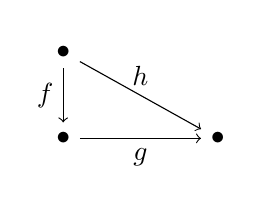
\begin{tikzpicture}[every node/.style={midway}]
      \matrix[column sep={5em,between origins}, row sep={2em}] at (0,0)
      {
        \node(A) {$\bullet$};\\
        \node(B) {$\bullet$}; & \node(C) {$\bullet$}; \\
      };

      \draw[->] (A) -- (B) node[anchor=east] {$f$};
      \draw[->] (B) -- (C) node[anchor=north]  {$g$};
      \draw[->] (A) -- (C) node[anchor=south] {$h$};
    \end{tikzpicture}
  \end{center}
  Primijetimo da objektima nismo dali imena (zato što nam to za ovaj primjer nije
  bitno), ali to ne znači da su ta tri objekta jednaka. Ako vrijedi:
  \begin{align*}
    g \circ f = h
  \end{align*}
  tada kažemo da dijagram \textbf{komutira}.
  Zakon asocijativnosti za $f, g, h$ dijagramom možemo prikazati kao:
  \begin{center}
    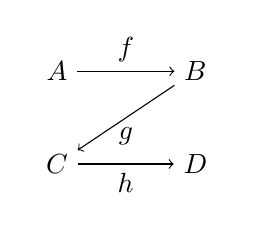
\begin{tikzpicture}[every node/.style={midway}]
      \matrix[column sep={5em,between origins}, row sep={2em}] at (0,0)
      {
        \node(A) {$A$}; & \node(B) {$B$}; \\
        \node(C) {$C$}; & \node(D) {$D$}; \\
      };
      \draw[->] (A) -- (B) node[anchor=south] {$f$};
      \draw[->] (B) -- (C) node[anchor=north] {$g$};
      \draw[->] (C) -- (D) node[anchor=north] {$h$};
    \end{tikzpicture}
  \end{center}


  Kao i u mnogim granama matematike, u teoriji kategorija ponekad želimo
  pokazati da su dvije stvari jednake. Rijetko želimo pokazati da su dva
  objekta jednaka; češće ćemo pokazivati jednakost strelica i za to ćemo
  koristiti tehniku zvanu praćenje dijagrama (eng. diagram chasing).
  Dijagram:

  \begin{center}
    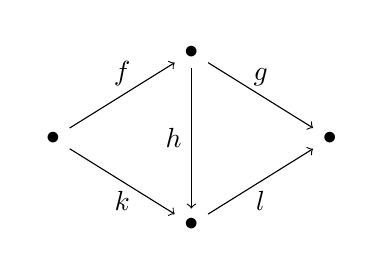
\begin{tikzpicture}[every node/.style={midway}]
      \matrix[column sep={5em,between origins}, row sep={2em}] at (0,0)
      {
        & \node(B) {$\bullet$}; &\\
        \node(A) {$\bullet$}; && \node(C) {$\bullet$}; \\
        & \node(D) {$\bullet$}; & \\
      };
      \draw[->] (A) -- (B) node[anchor=south] {$f$};
      \draw[->] (B) -- (C) node[anchor=south] {$g$};
      \draw[->] (B) -- (D) node[anchor=east] {$h$};
      \draw[->] (A) -- (D) node[anchor=north] {$k$};
      \draw[->] (D) -- (C) node[anchor=north] {$l$};
    \end{tikzpicture}
  \end{center}
  ima četiri neimenovana objekta, pet strelica ($f, g, h, k, l$) i pet
  strelica nastalih kompozicijom:
  \begin{align*}
    g \circ f, h \circ f, l \circ h \circ f, l \circ h, l \circ k
  \end{align*}
  Primijetimo da neke od tih strelica mogu biti jednake.
  Ovaj dijagram ima tri ćelije: vanjsku $(f, k, l, g)$, lijevi
  unutarnji trokut $(f, h, k)$ i desni unutarnji trokut $(h, g, l)$.
  Neke od tih ćelija mogu komutirati:
  \begin{itemize}
      \item lijevi trokut komutira ako vrijedi $h \circ f = k$
      \item desni trokut komutira ako vrijedi $l \circ h = g$
      \item vanjska ćelija komutira ako vrijedi $g \circ f = l \circ k$
  \end{itemize}
  Praćenje dijagrama je proces u kojem pokazujemo da neka ćelija komutira pomoću
  činjenica da neke druge ćelije komutiraju te nekih drugih svojstava dijagrama.

  \primjer{
    Pokažimo za prethodni dijagram da ukoliko unutarnji trokuti
    komutiraju, tada vanjska ćelija komutira tj. ako vrijedi:
    \begin{align*}
      h \circ f = k \qquad  l \circ h = g
    \end{align*}
    tada vrijedi:
    \begin{align*}
      g \circ f = l \circ k.
    \end{align*}
    Pokažimo to algebarski:
    \begin{align*}
      g \circ f = (l \circ h) \circ f \overset{(\ref{def:kat_assoc})}{=} l \circ (h \circ f) = l \circ k
    \end{align*}
    Tehnikom praćenja dijagrama i uočavanjem da su neke kompozicije jednake
    imamo:
    \begin{center}
      \begin{tikzpicture}[every node/.style={midway}]
        \matrix[column sep={3em,between origins}, row sep={1em}, ampersand replacement=\&] at (0,0)
        {
          \& \node(B) {$\bullet$}; \&\&\&\& \node(E) {$\bullet$}; \&\&\&\&\&\\
          \node(A) {$\bullet$}; \&\& \node(C) {$\bullet$}; \& \node(EQ1) {$=$};
          \& \node(D) {$\bullet$}; \&\& \node(G) {$\bullet$}; \& \node(EQ2) {$=$};
          \& \node(I) {$\bullet$}; \&\& \node(K) {$\bullet$};\\
          \&\&\&\&\& \node(F) {$\bullet$}; \&\&\&\& \node(J) {$\bullet$}; \& \\
        };
      \draw[->] (A) -- (B) node[anchor=south] {$f$};
      \draw[->] (B) -- (C) node[anchor=south] {$g$};
      \draw[->] (D) -- (E) node[anchor=south] {$f$};
      \draw[->] (E) -- (F) node[anchor=east] {$h$};
      \draw[->] (F) -- (G) node[anchor=north] {$l$};
      \draw[->] (I) -- (J) node[anchor=north] {$k$};
      \draw[->] (J) -- (K) node[anchor=north] {$l$};
      \end{tikzpicture}
    \end{center}
  }

  Kod jednostavnijih primjera ne vidi se prednost korištenja tehnike dijagrama.
  Pokažimo sada na malo kompliciranijem primjeru kako se tehnikom dijagrama
  intuitivnije može objasniti komutacija dijagrama.

  \primjer{
    Ako u dijagramu:
    \begin{center}
      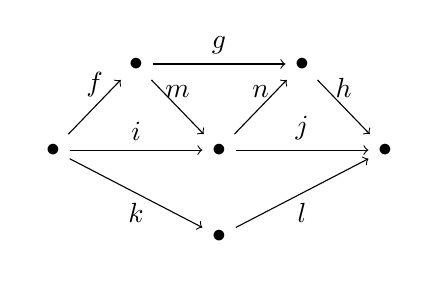
\begin{tikzpicture}[every node/.style={midway}]
        \matrix[column sep={3em,between origins}, row sep={2em}, ampersand replacement=\&] at (0,0)
        {
          \& \node(B) {$\bullet$};\&\&  \node(C) {$\bullet$}; \&\\
          \node(A) {$\bullet$}; \&\& \node(E) {$\bullet$}; \&\& \node(D) {$\bullet$};\\
          \&\& \node(F) {$\bullet$}; \&\&\\
        };
      \draw[->] (A) -- (B) node[anchor=south] {$f$};
      \draw[->] (B) -- (C) node[anchor=south] {$g$};
      \draw[->] (C) -- (D) node[anchor=south] {$h$};
      \draw[->] (A) -- (E) node[anchor=south] {$i$};
      \draw[->] (E) -- (D) node[anchor=south] {$j$};
      \draw[->] (B) -- (E) node[anchor=south] {$m$};
      \draw[->] (E) -- (C) node[anchor=south] {$n$};
      \draw[->] (A) -- (F) node[anchor=north] {$k$};
      \draw[->] (F) -- (D) node[anchor=north] {$l$};
      \end{tikzpicture}
    \end{center}

    \noindent komutiraju četiri unutarnja trokuta, pokažimo da komutira i vanjska
    ćelija. Cilj nam je pokazati da vrijedi:
    \begin{center}
      $h \circ g \circ f = l \circ k$
    \end{center}
    Algebarski:
    \begin{align*}
      h \circ g \circ f &= h \circ (n \circ m) \circ f = (h \circ n) \circ (m \circ f) =\\
      &= j \circ i = l \circ k\\
    \end{align*}
    Pokažimo to tehnikom praćenja dijagrama.
    \begin{center}
      \begin{tikzpicture}[every node/.style={midway}]
        \matrix[column sep={3em,between origins}, row sep={2em}, ampersand replacement=\&] at (0,0)
        {
          \node(EQ3) {$\quad$}; \&\& \node(B) {$\bullet$};\&\&  \node(C) {$\bullet$}; \&\&
          \&\& \node(B1) {$\bullet$};\&\&  \node(C1) {$\bullet$}; \&\\
          \&\node(A) {$\bullet$}; \&\& ; \&\& \node(D) {$\bullet$}; \& \node(EQ1) {$=$};
          \& \node(A1) {$\bullet$}; \&\& \node(E1) {$\bullet$}; \&\& \node(D1)
          {$\bullet$}; \& \node(EQ2) {$=$};\\
        };
      \draw[->] (A) -- (B) node[anchor=south] {$f$};
      \draw[->] (B) -- (C) node[anchor=south] {$g$};
      \draw[->] (C) -- (D) node[anchor=south] {$h$};

      \draw[->] (A1) -- (B1) node[anchor=south] {$f$};
      \draw[->] (C1) -- (D1) node[anchor=south] {$h$};
      \draw[->] (B1) -- (E1) node[anchor=south] {$m$};
      \draw[->] (E1) -- (C1) node[anchor=south] {$n$};

      \end{tikzpicture}
    \end{center}
    \begin{center}
      \begin{tikzpicture}[every node/.style={midway}]
        \matrix[column sep={3em,between origins}, row sep={2em}, ampersand replacement=\&] at (0,0)
        {
          \node(EQ2) {$=$}; \& \node(A) {$\bullet$}; \&\& \node(E) {$\bullet$}; \&\& \node(D)
          {$\bullet$}; \& \node(EQ1) {$=$};
          \& \node(A1) {$\bullet$}; \&\& \&\& \node(D1) {$\bullet$}; \&\\
          \&\&\&\&\&\&\&\&\& \node(F1) {$\bullet$}; \&\&\\
        };
      \draw[->] (A) -- (E) node[anchor=south] {$i$};
      \draw[->] (E) -- (D) node[anchor=south] {$j$};
      \draw[->] (A1) -- (F1) node[anchor=south] {$k$};
      \draw[->] (F1) -- (D1) node[anchor=south] {$l$};
      \end{tikzpicture}
    \end{center}

  }
  %%%%%%%%%%%%%%%%%%%
  %% Monoik i epik %%
  %%%%%%%%%%%%%%%%%%%
  \newpage
  \section{Monoik i epik}
  U ovom poglavlju proširujemo terminologiju i proučavamo posebne slučajeve
  strelica kako bismo došli do definicije izomorfizma.
  \begin{definition}
    U proizvoljnoj kategoriji \category{G} strelicu:
    \begin{align*}
      B \xrightarrow{m} A
    \end{align*}
    za koju vrijedi da za svaki par strelica
    \begin{align*}
      X \xbigtoto[g]{f} B
    \end{align*}
    vrijedi:
    \begin{align}
      m \circ f = m \circ g \implies f = g
    \end{align}
    zovemo \textbf{monoik}.
  \end{definition}
  \primjer{
    Neka je \category{G} neka kategorija na skupovima i neka su strelice
    totalne funkcije između skupova.
    Ako je $B \xrightarrow{m} A$ injektivna (kao funkcija) tada je $m$ monoik (kao
    strelica). Pokažimo to.\\
    Pretpostavimo da vrijedi:
    \begin{align} \label{me:pr:1}
      m \circ f = m \circ g
    \end{align}
    za neki paralelni par strelica
    \begin{align*}
      A \xbigtoto[g]{f} B
    \end{align*}
    Kako su $f$ i $g$ totalne funkcije dovoljno je pokazati da za svaki $x \in X$
    vrijedi:
    \begin{align*}
      f(x) = g(x)
    \end{align*}
    Imamo:
    \begin{align*}
      m(f(x)) = (m \circ f)(x) \overset{(\ref{me:pr:1})}{=} (m \circ g)(x) = m(g(x))
    \end{align*}
    No, kako je $m$ injektivna za $a, b \in B$ imamo:
    \begin{align*}
      m(a) = m(b) \implies a = b
    \end{align*}
    pa je $m$ monoik.
  }

  \begin{definition}
    U proizvoljnoj kategoriji \category{G} strelicu:
    \begin{align*}
      A \xrightarrow{e} B
    \end{align*}
    za koju vrijedi da za svaki par strelica
    \begin{align*}
      B \xbigtoto[g]{f} X
    \end{align*}
    vrijedi:
    \begin{align}
      f \circ e = g \circ e \implies f = g
    \end{align}
    zovemo \textbf{epik}.
  \end{definition}
  Pokažimo sada na sličnom primjeru kao i ranije kako se epik ponaša na
  kategoriji nad skupovima.
  \primjer{
    Neka je \category{G} neka kategorija na skupovima i neka su strelice
    totalne funkcije između skupova.
    Ako je $A \xrightarrow{e} B$ surjektivna (kao funkcija) tada je epik (kao
    strelica).
    Pretpostavimo da vrijedi:
    \begin{align} \label{me:pr:2}
      f \circ e = g \circ e
    \end{align}
    za neki paralelni par strelica
    \begin{align*}
      B \xbigtoto[g]{f} X
    \end{align*}
    Kako su $f$ i $g$ totalne funkcije dovoljno je pokazati da za $x \in X$
    vrijedi:
    \begin{align*}
      f(x) = g(x)
    \end{align*}
    Kako je $e$ surjektivna znamo da za $b \in B$ postoji $a \in A$ takav da
    vrijedi:
    \begin{align*}
      b = e(a)
    \end{align*}
    Imamo:
    \begin{align*}
      f(b) = f(e(a)) = (f \circ e)(a) = (g \circ e)(a) = g(e(a)) = g(b)
    \end{align*}
    Pa je $e$ epik.
  }
    Prethodni primjeri pokazuju da za "dovoljno lijepe" kategorije vrijedi:
    \begin{center}
      injekcija $\implies$ monoik \qquad surjekcija $\implies$ epik
    \end{center}
    No, za neke kategorije "injektivna strelica" ili "surjektivna strelica"
    nemaju smisla tako da takva intuitivna interpretacija ima smisla samo za
    "dovoljno lijepe" kategorije. Pravilnije bi bilo gledati na monoik i epik
    kao na strelice koje se mogu "poništiti" na jednoj strani. Ako pak strelica
    ima jednostrani inverz tada dobivamo posebnu klasu monoika i epika.
    \begin{definition}
      Ako za strelice:
      \begin{align*}
        B \xrightarrow{s} A, \qquad A \xrightarrow{r} B
      \end{align*}
      vrijedi:
      \begin{align*}
        r \circ s = id_B
      \end{align*}
      tada $s$ nazivamo \textbf{sekcija}, a $r$ \textbf{retrakcija}.
    \end{definition}
    Lako se pokaže da je svaka sekcija monoik i svaka retrakcija epik.
    \begin{definition}
      \textbf{Bimorfizam} je strelica koja je monik i epik.
    \end{definition}
    \begin{definition}
      Za strelicu $A \xrightarrow{f} B$ kažemo da je \textbf{izomorfizam} ako
      postoji strelica $B \xrightarrow{g} A$ takva da vrijedi:
      \begin{align}
        g \circ f = id_A \wedge f \circ g = id_B
      \end{align}
    \end{definition}
    \begin{definition}
      Za dva objekta $A$ i $B$ kažemo da su \textbf{izomorfni} ako postoji izomorfizam
      $A \xrightarrow{} B$.
    \end{definition}

    Lako se pokaže da ukoliko je strelica sekcija i epik ili retrakcija i
    monoik tada je i izomorfizam.
    Grafički prikazano:
    \begin{center}
    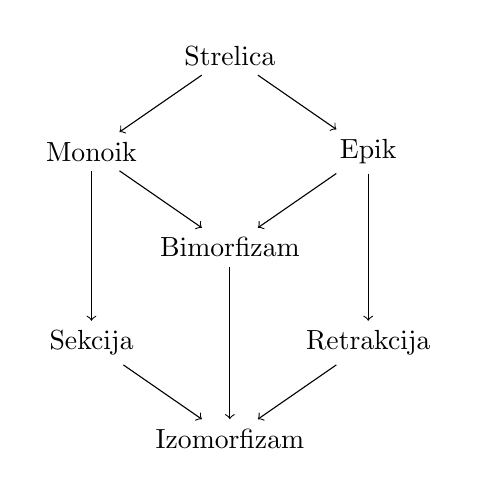
\begin{tikzpicture}[every node/.style={midway}]
      \matrix[column sep={5em,between origins}, row sep={2em}] at (0,0)
      {
        & \node(S) {Strelica}; &\\
        \node(M) {Monoik}; && \node(E) {Epik}; \\
        & \node(B) {Bimorfizam}; & \\
        \node(SM) {Sekcija}; && \node(SE) {Retrakcija};\\
        & \node(I) {Izomorfizam}; & \\
      };
      \draw[->] (S) -- (M) node[anchor=north] {};
      \draw[->] (S) -- (E) node[anchor=north] {};
      \draw[->] (E) -- (SE) node[anchor=north] {};
      \draw[->] (E) -- (B) node[anchor=north] {};
      \draw[->] (M) -- (SM) node[anchor=north] {};
      \draw[->] (M) -- (B) node[anchor=north] {};
      \draw[->] (SM) -- (I) node[anchor=north] {};
      \draw[->] (SE) -- (I) node[anchor=north] {};
      \draw[->] (B) -- (I) node[anchor=north] {};
    \end{tikzpicture}
    \end{center}
  %%%%%%%%%%%%%%%%%%%%%%%%%%%%%%%
  %% Kategorijski konstruktori %%
  %%%%%%%%%%%%%%%%%%%%%%%%%%%%%%%
  \newpage
  \section{Kategorijski konstrukori}
  U ovom poglavlju istražujemo neke osnovne kategorijske
  konstruktore, tj. objekte koji zadovoljavaju neka pravila definirana u teoriji
  kategorija. Kako u jeziku kategorija ne gledamo unutrašnju strukturu objekata
  svi koncepti moraju biti definirani pomoću relacija između objekata.
  \subsection{Inicijalni i finalni objekti}
  \begin{definition}
    Za objekt $S$ u kategoriji \category{G} kažemo da je \textbf{inicijalni} ako za svaki
    objekt $A$ postoji jedinstvena strelica $S \xrightarrow{} A$.
  \end{definition}
  \begin{definition}
    Za objekt $S$ u kategoriji \category{G} kažemo da je \textbf{finalni} ako za svaki
    objekt $A$ postoji jedinstvena strelica $A \xrightarrow{} S$.
  \end{definition}
  Lako se pokaže da ukoliko je objekt $I$ finalni objekt u kategoriji \category{G} tada je $I$ inicijalni objekt u $\category{G}^{op}$.
  \primjer{
    Neka je \category{Set} kategorija skupova i neka je 
    \begin{center}
      $1 = \{x\}$
    \end{center}
    skup s jednim elementom. Za svaki skup $A$ postoji jedinstvena strelica
    \begin{center}
      $A \xrightarrow{} 1$
    \end{center}
    (funkcija koja preslikava sve u $x$) pa je $1$ finalni objekt za
    \category{Set}.
    Za svaki skup $A$ postoji jedinstvena strelica
    \begin{center}
      $\emptyset \xrightarrow{} A$
    \end{center}
    (gdje je $\emptyset$ prazan skup) pa je $\emptyset$ inicijalni objekt za
    \category{Set}.
  }
  \primjer{ \codei{Void} je inicijalni objekt u \category{Hask}.
    Zbog polimorfizma \footnote{Parametrizirani polimorfizam omogućava da se
      funkcije pišu generalno bez ovisnosti o tipu, opširnije o tome u
      poglavlju "Funktori". Za sada možemo funkciju \codei{absurd :: -> a}
      interpretirati kao skup funkcija \{Void $\to$ a $|$ a je tip u
      \category{Hask}\} čije pozivanje ovisi o kodomeni.} možemo definirati polimorfnu funkciju:
    \code{
      absurd :: Void -> a
    }
    gdje je \codei{a} bilo koji tip u \category{Hask}.
  }
  \primjer{ \codei{()} je finalni objekt u \category{Hask}.
    Možemo definirati polimorfnu funkciju \codei{unit :: a -> ()} kao:
    \code{
      unit x = ()
    }
  }
  Kategorija \category{C} može imati i finalni i inicijalni objekt, a ako ima
  oboje onda oni ne moraju biti isti. Objekt koji je i finalni i inicijalni ponekad
  zovemo \textbf{nulti} objekt. Lako se pokaže da ukoliko kategorija ima dva inicijalna
  objekta tada su oni izomorfni. Stoga ima smisla govoriti o inicijalnom objektu
  kategorije te analogno o finalnom objektu.
  \subsection{Produkti i koprodukti}
  Produkt u teoriji kategorija je generalizacija Kartezijskog produkta na
  skupovima. Prisjetimo se, ako su $A, B$ skupovi tada je Kartezijev produkt ta
  dva skupa:
  \begin{align*}
    A \times B = \{ (a, b) | a \in A, b \in B\}
  \end{align*}
  Primijetimo da je uz takvu definiciju Kartezijevog produkta prirodno
  definirati dvije projekcije:
  \begin{align*}
    p_A &: A \times B \to A, p_A(a, b) = a\\
    p_B &: A \times B \to B, p_B(a, b) = b\\
  \end{align*}
  Ako su \codei{a} i \codei{b} proizvoljni tipovi u \category{Hask} te dvije
  funkcije zovemo \codei{fst} i \codei{snd}.
  \begin{mcode}
    fst :: (a, b) -> a
    fst (x, y) = x

    snd :: (a, b) -> b
    snd (x, y) = y
  \end{mcode}
  Pa na razini kategorija definiramo prvi konstruktor.
  \begin{definition}
    Za $A, B \in Obj_C$ \textbf{grananje prema paru $A, B$} je objekt $X \in
    Obj_C$
    zajedno sa strelicama:
  \begin{center}
    \begin{tikzpicture}[every node/.style={midway}]
      \matrix[column sep={3em,between origins}, row sep={2em}] at (0,0)
      {
        && \node(A) {$A$}; \\
        \node(X) {$X$};\\
        && \node(B) {$B$};\\
      };
      \draw[->] (X) -- (A) node[anchor=south] {};
      \draw[->] (X) -- (B) node[anchor=south] {};
    \end{tikzpicture}
  \end{center}
  \end{definition}
  \begin{definition}
    Za $A, B \in Obj_C$ \textbf{grananje od para $A, B$} je objekt $X \in
    Obj_C$
    zajedno sa strelicama:
  \begin{center}
    \begin{tikzpicture}[every node/.style={midway}]
      \matrix[column sep={3em,between origins}, row sep={2em}] at (0,0)
      {
        \node(A) {$A$}; \\
        && \node(X) {$X$};\\
        \node(B) {$B$};\\
      };
      \draw[->] (A) -- (X) node[anchor=south] {};
      \draw[->] (B) -- (X) node[anchor=south] {};
    \end{tikzpicture}
  \end{center}
  \end{definition}
  Kada će iz konteksta biti jasno o kojem grananju se radi, govorit ćemo
  samo o grananju. Sada možemo definirati produkt.
  \begin{definition}
    Neka su $A, B \in Obj_C$. \textbf{Produkt} od $A$ i $B$ je grananje
  \begin{center}
    \begin{tikzpicture}[every node/.style={midway}]
      \matrix[column sep={3em,between origins}, row sep={2em}] at (0,0)
      {
        && \node(A) {$A$}; \\
        \node(S) {$S$};\\
        && \node(B) {$B$};\\
      };
      \draw[->] (S) -- (A) node[anchor=south] {$p_A$};
      \draw[->] (S) -- (B) node[anchor=north] {$p_B$};
    \end{tikzpicture}
  \end{center}
  sa svojstvom da za svako grananje:
  \begin{center}
    \begin{tikzpicture}[every node/.style={midway}]
      \matrix[column sep={3em,between origins}, row sep={2em}] at (0,0)
      {
        && \node(A) {$A$}; \\
        \node(X) {$X$};\\
        && \node(B) {$B$};\\
      };
      \draw[->] (X) -- (A) node[anchor=south] {$f_A$};
      \draw[->] (X) -- (B) node[anchor=north] {$f_B$};
    \end{tikzpicture}
  \end{center}
  postoji jedinstvena strelica $X \xrightarrow{m} S$ takva da dijagram:
  \begin{center}
    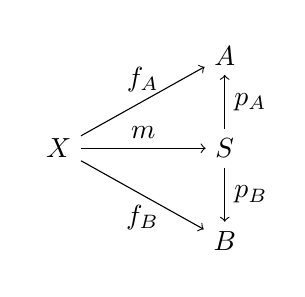
\begin{tikzpicture}[every node/.style={midway}]
      \matrix[column sep={3em,between origins}, row sep={2em}] at (0,0)
      {
        && \node(A) {$A$}; \\
        \node(X) {$X$}; && \node(S) {$S$};\\
        && \node(B) {$B$};\\
      };
      \draw[->] (X) -- (A) node[anchor=south] {$f_A$};
      \draw[->] (X) -- (B) node[anchor=north] {$f_B$};
      \draw[->] (X) -- (S) node[anchor=south] {$m$};
      \draw[->] (S) -- (A) node[anchor=west] {$p_A$};
      \draw[->] (S) -- (B) node[anchor=west] {$p_B$};
    \end{tikzpicture}
  \end{center}
  komutira. Tada $m$ zovemo \textbf{mediator} za grananje na $X$.
  \end{definition}
  Primijetimo dvije stvari:
  \begin{itemize}
    \item produkt nije samo objekt, produkt je objekt i dvije strelice
    \item mediator je jedinstveni za grananje na $X$
  \end{itemize}
  U \category{Hask}-u možemo definirati funkciju (višeg reda)
  \codei{factorizer} koja će za bilo koji tip c i dvije projekcije $c
  \xrightarrow{p} a$ i $c \xrightarrow{q} b$ vratiti jedinstveni mediator.
  \begin{mcode}
    factorizer :: (c -> a) -> (c -> b) -> (c -> (a, b))
    factorizer p q = \x -> (p x, q x)
  \end{mcode}
  Analogno definiramo i koprodukt.

  \begin{definition}
    Neka su $A, B \in Obj_C$. \textbf{Koprodukt} od $A$ i $B$ je grananje
  \begin{center}
    \begin{tikzpicture}[every node/.style={midway}]
      \matrix[column sep={3em,between origins}, row sep={2em}] at (0,0)
      {
        \node(A) {$A$}; \\
        && \node(X) {$S$};\\
        \node(B) {$B$};\\
      };
      \draw[->] (A) -- (X) node[anchor=south] {$i_A$};
      \draw[->] (B) -- (X) node[anchor=north] {$i_B$};
    \end{tikzpicture}
  \end{center}
  sa svojstvom da za svako grananje:
  \begin{center}
    \begin{tikzpicture}[every node/.style={midway}]
      \matrix[column sep={3em,between origins}, row sep={2em}] at (0,0)
      {
        \node(A) {$A$}; \\
        && \node(X) {$X$};\\
        \node(B) {$B$};\\
      };
      \draw[->] (A) -- (X) node[anchor=south] {$f_A$};
      \draw[->] (B) -- (X) node[anchor=north] {$f_B$};
    \end{tikzpicture}

  \end{center}
  postoji jedinstvena strelica $S \xrightarrow{m} X$ takva da dijagram:
  \begin{center}
    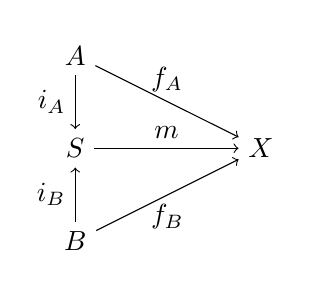
\begin{tikzpicture}[every node/.style={midway}]
      \matrix[column sep={3em,between origins}, row sep={2em}] at (0,0)
      {
        \node(A) {$A$}; \\
        \node(S) {$S$}; && \node(X) {$X$};\\
        \node(B) {$B$};\\
      };
      \draw[->] (A) -- (X) node[anchor=south] {$f_A$};
      \draw[->] (B) -- (X) node[anchor=north] {$f_B$};
      \draw[->] (A) -- (S) node[anchor=east] {$i_A$};
      \draw[->] (B) -- (S) node[anchor=east] {$i_B$};
      \draw[->] (S) -- (X) node[anchor=south] {$m$};
    \end{tikzpicture}
  \end{center}
  komutira.
  \end{definition}

  \begin{definition}
    Za kategoriju \category{C} kažemo da je \textbf{Kartezijeva} (skraćeno
    \category{C} je \textbf{CC}) ako:
    \begin{itemize}
      \item sadrži inicijalni objekt,
      \item za svaki par $A, B \in Obj_C$ postoji Kartezijev produkt.
    \end{itemize}
  \end{definition}
  \primjer{
    Za kategoriju \category{Set} već smo pokazali da sadrži inicijalni objekt
    $\emptyset$.
    Pokažimo sada da je Kartezijev produkt i produkt u kategorijskom smislu.
    Neka su $A$ i $B$ skupovi.
    Za proizvoljno grananje
    \begin{center}
      \begin{tikzpicture}[every node/.style={midway}, ampersand replacement=\&]
        \matrix[column sep={3em,between origins}, row sep={2em}] at (0,0)
        {
          \&\& \node(A) {$A$}; \\
          \node(X) {$X$};\\
          \&\& \node(B) {$B$};\\
        };
        \draw[->] (X) -- (A) node[anchor=south] {$f_A$};
        \draw[->] (X) -- (B) node[anchor=north] {$f_B$};
      \end{tikzpicture}
    \end{center}
    na X definiramo $X \xrightarrow{m} A \times B$ kao:
    \begin{align*}
      m(x) = (f_A(x), f_B(x))
    \end{align*}
    za $x \in X$. Lako se pokaže da sljedeći dijagram komutira:
  \begin{center}
    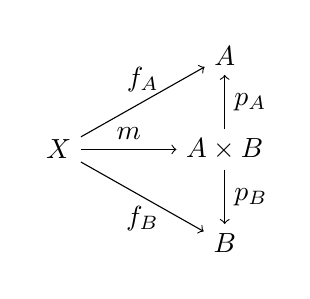
\begin{tikzpicture}[every node/.style={midway}]
      \matrix[column sep={3em,between origins}, row sep={2em}, ampersand replacement=\&] at (0,0)
      {
        \&\& \node(A) {$A$}; \\
        \node(X) {$X$}; \&\& \node(S) {$A \times B$};\\
        \&\& \node(B) {$B$};\\
      };
      \draw[->] (X) -- (A) node[anchor=south] {$f_A$};
      \draw[->] (X) -- (B) node[anchor=north] {$f_B$};
      \draw[->] (X) -- (S) node[anchor=south] {$m$};
      \draw[->] (S) -- (A) node[anchor=west] {$p_A$};
      \draw[->] (S) -- (B) node[anchor=west] {$p_B$};
    \end{tikzpicture}
  \end{center}
  Ostaje nam pokazati jedinstvenost, tj. da je $m$ jedina takva funkcija.
  Pretpostavimo da postoji neka druga funkcija
  \begin{align*}
    X \xrightarrow{h} A \times B
  \end{align*}
  takva da  vrijedi:
  \begin{align*}
    p_A \circ h = f_A \qquad p_B \circ h = f_B\\
  \end{align*}
  Za $x \in X$ imamo:
  \begin{align*}
    h(x) = (p_A(h(x), p_B(h(x))) = ((p_A \circ h )(x), (p_B \circ h)(x)) =
    (f_A(x), f_B(x)) = m(x)
  \end{align*}
  Pa je \category{Set} jedna Kartezijeva kategorija.
  }
  \newpage

  %%%%%%%%%%%%%%
  %% Funktori %%
  %%%%%%%%%%%%%%
  \section{Funktori}
  Do sada smo definirali kategorije, posebno i \category{Hask} kategoriju,
  proučavali različite vrste strelica, objekata i pokazali njihove ekvivalente
  u \category{Hask}-u. U ovom poglavlju bavimo se "preslikavanjima" između
  kategorija i demonstriramo praktičnu primjenu teorije kategorije u Haskellu.
  \begin{definition}
    Neka su \category{C} i \category{G} kategorije. \textbf{Funktor} $F$ iz
    \category{C} u \category{G} je preslikavanje koje:
    \begin{itemize}
      \item svakome $x \in Obj_\category{C}$ pridružuje $F(x) \in
        Obj_\category{G}$
      \item svakome $X \xrightarrow{f} Y \in Arw_\category{C}$ pridružuje
        $F(X) \xrightarrow{F(f)} F(Y) \in Arw_\category{G}$ tako da vrijedi:
        \begin{itemize}
          \item $F(id_X) = id_{F(X)}$ za $X \in Obj_\category{C}$
          \item $F(g \circ f) = F(g) \circ F(f)$ za sve $X \xrightarrow{f} Y$ i
            $Y \xrightarrow{g} Z$
        \end{itemize}
    \end{itemize}
  \end{definition}
  Funktori čuvaju strukturu kategorije, odnosno sve što je povezano u početnoj
  kategoriji ostat će povezano i u krajnjoj.
  \begin{definition}
    Neka je \category{C} proizvoljna kategorija i neka je $F$ funktor sa
    \category{C} u \category{C}. Tada kažemo da je $F$ \textbf{endofunktor} nad
    \category{C}.
  \end{definition}
  \primjer{
    Neka je \category{C} proizvoljna kategorija te neka je $F$ preslikavanje
    iz \category{C}  u \category{C} takvo da vrijedi:
    \begin{itemize}
      \item $x = F(x)$ za svaki $x \in Obj_\category{C}$
      \item $f = F(f)$ za svaki $f \in Obj_\category{C}$
    \end{itemize}
    Tada je $F$ endofunktor nad \category{C} koji zovemo \textbf{funktor identitete}.
  }
  Funktori u Haskellu usko su povezani sa gornjom definicijom funktora. 
  Da bismo mogli objasniti funktore u Haskellu na primjeru napravit ćemo malu digresiju i definirati
  jedan od najjednostavnijih parametriziranih tipova: \codei{Maybe}
  \subsection{Maybe}
  Parametrizirani tip \codei{Maybe} služi za enkapsuliranje opcionalnih
  vrijednosti, na primjer pretpostavimo da želimo napisati funkciju u Haskellu koja će
  dohvatiti prvi element liste cijelih brojeva. Što će se dogoditi ako je lista prazna?

  Tip \codei{Maybe} omogućava nam da modeliramo tip koji može ali i ne mora
  imati vrijednost. Isto kao što tip \codei{Bool} može imati \codei{True}
  ili \codei{False} tako \codei{Maybe} može imati vrijednosti \codei{Just a} ili
  \codei{Nothing}. Primijetimo da, iako formalno \codei{Maybe} može imati dvije
  vrijednosti, prirodno je vrijednost \codei{Nothing} interpretirati kao da nismo dobili ništa (što može
  služiti za rješavanje takozvanih rubnih uvjeta).

  \codei{Maybe} je parametrizirani konstruktor tipa, što znači da pomoću njega možemo generirati nove tipove. Definicija \codei{Maybe} u
  Haskellu:
  \begin{mcode}
    data Maybe a = Just a | Nothing
  \end{mcode}
  Vidimo da pomoću \codei{Maybe a}, gdje je \codei{a} bilo koji tip možemo
  konstruirati druge tipove koji mogu imati vrijednost ili \codei{Just a} ili
  \codei{Nothing}. Npr. \codei{Maybe Integer} može imati vrijednost \codei{Just
    Integer} ili \codei{Nothing}. Vratimo li se na primjer liste, to znači da naša funkcija
  koja bi vraćala prvi element liste cijelih brojeva ima tip:
  \begin{mcode}
    head' :: [Integer] -> Maybe Integer
  \end{mcode}
  Kada pozovemo \codei{head} na praznoj listi dobijemo \codei{Nothing}, dok na
  nepraznoj dobijemo \codei{Just Int}, npr.
  \begin{mcode}
    >> head' [2, 4, 6, 8, 10]
    Just 2
    >> head' []
    Nothing
  \end{mcode}
  \subsection{Funktori u Haskellu}
  Kako se funktor sastoji od dva dijela: preslikava objekte iz jedne kategorije u drugu
  i preslikava strelice iz prve kategorije u drugu, funktori u Haskellu su iz
  \category{Hask} u \category{Func}, gdje je \category{Func} potkategorija od
  \category{Hask}-a. Funktor liste ide iz \category{Hask} u \category{Lst},
  gdje \category{Lst} sadrži samo liste, tj.\codei{[T]}\footnote{
    \codei{[a]} je konstruktor tipa sa jednim parametrom,
    kao i \codei{Maybe a}}
  za bilo koji tip \codei{T}. Definicija funktora u Haskellu:
  \begin{mcode}
    class Functor (f :: * -> *) where
      fmap :: (a -> b) -> f a -> f b
  \end{mcode}
  koji mora zadovoljavati:
  \begin{mcode}
    fmap id = id
    fmap (f . g) = fmap f . fmap g
  \end{mcode}
  Primijetimo da su ti uvjeti u skladu sa definicijom funktora u kategoriji.
  \primjer{
    Pokažimo da je \codei{Maybe a} funktor.
    Primijetimo da, pošto je \codei{Maybe} konstruktor tipa (s jednim
    parametrom), bilo koji tip \codei{X} možemo poslati iz \category{Hask}-a i
    dobiti novi tip \codei{Maybe X}. Zaključujemo da \codei{Maybe}
    preslikava objekte iz jedne kategorije u drugu\footnote{Objekti u
      kategoriji \category{Hask} su tipovi}.

    Definirajmo sada \codei{fmap} kako bi bili zadovoljeni ostali uvjeti da
    \codei{Maybe a} bude funktor.
    \begin{mcode}
      instance Functor Maybe where
        fmap f (Just x) = Just (f x)
        fmap f Nothing = Nothing
    \end{mcode}
    Iz gornje definicije vidimo da za bilo koji \codei{A} $\xrightarrow{f}$
    \codei{B} $\in
    Arw_\category{Hask}$ vrijedi: \codei{Maybe A}
    $\xrightarrow{\texttt{fmap f}}$ \codei{Maybe B}.
    Lako se provjeri da sa tako definiranom funkcijom \codei{fmap} 
    \codei{Maybe a} jest funktor.
  }
  Korisna intuicija kod Haskellovih funktora je da oni reprezentiraju tipove
  preko kojih se može mapirati: to mogu biti liste cijelih brojeva,
  balansirana stabla, opcionalne vrijednosti (\codei{Maybe a}) ili nešto drugo.

  Jednostavan primjer mapiranja preko liste cijelih brojeva može se pokazati
  korištenjem funkcije \codei{double} koja će udvostručiti cijeli broj.
  Definicija \codei{double} u Haskellu:
  \begin{mcode}
    double :: Double -> Double
    double n = n * 2
  \end{mcode}
  Primijetimo da \codei{double} možemo gledati kao \codei{Double}
  $\xrightarrow{\texttt{double}}$ \codei{Double}. Kako je lista cijelih
  brojeva (\codei{[Double]}) funktor, možemo preslikati \codei{double} 
  u \codei{[Double]} $\xrightarrow{\texttt{fmap double}}$
  \codei{[Double]}. Npr.:
  \begin{mcode}
    >> fmap double [1.0..10.0]
    [2.0,4.0,6.0,8.0,10.0,12.0,14.0,16.0,18.0,20.0]
  \end{mcode}
  Time smo preko teorije kategorije funktora eliminirali potrebu za
  petljama koje su neizostavne kod imperativnih programskih jezika.
  \newpage
  \section*{Literatura}
  \begin{description}
    \item[[1]]
      Harold Simmons, An Introduction to Category Theory,
      \url{http://www.cs.man.ac.uk/~hsimmons/zCATS.pdf}
    \item[[2]]
      Michael Barr and Charles Wells, Category Theory for Computing
      Science,
      \url{http://www.tac.mta.ca/tac/reprints/articles/22/tr22.pdf}
    \item[[3]]
      \url {https://en.wikibooks.org/wiki/Haskell/Category\_theory}
    \item[[4]]
      \url {https://wiki.haskell.org/Type}

    \item[[5]] \label{bib:fast-loose}
      Nils Anders Danielsson, John Hughes, Patrik Jansson, Jeremy Gibbons,
Fast and Loose Reasoning is Morally Correct
\url{http://www.cs.ox.ac.uk/jeremy.gibbons/publications/fast+loose.pdf}
  \item[[6]]
    \url{http://bartoszmilewski.com/2014/11/24/types-and-functions/}
  \item[[7]]
    \url{http://bartoszmilewski.com/2015/01/07/products-and-coproducts/}
  \item[[8]]
    \url{http://bartoszmilewski.com/2015/01/20/functors/}
  \item[[9]]
    Pierce, Benjamin C. (2002). Types and Programming Languages.
  \end{description}
\end{document}
